\documentclass[11pt,a4paper]{article}
\usepackage[margin=1in]{geometry}
\usepackage{graphicx}
\usepackage{longtable}
\usepackage{hyperref}
\usepackage{booktabs}
\usepackage{enumitem}
\usepackage{titlesec}
\usepackage{lscape} % Added for rotating the image

% Format section titles
\titleformat{\section}{\bfseries\large}{\thesection}{1em}{}
\titleformat{\subsection}{\bfseries}{\thesubsection}{1em}{}

\hypersetup{colorlinks=true, linkcolor=blue}

\begin{document}

\begin{center}
  {\LARGE \bfseries Emotion‐Aware, Agentic Healthcare Chatbot Proposal} \\
  \vspace{0.5em}
  {Prepared by: Rishabh Gupta \quad | \quad July 2025}
\end{center}

\vspace{1em}

\section{Problem Statement}
Modern tele‐health interactions lack two critical capabilities:
\begin{enumerate}[left=0pt,label=\arabic*)]
  \item \textbf{Emotional Intelligence:} Traditional chatbots “hear” what patients say but ignore how they say it—anxiety and distress go unnoticed.
  \item \textbf{Modular Expertise \& Memory:} Monolithic dialogue models struggle with medical accuracy and conversational empathy, and lack persistent memory across sessions.
\end{enumerate}

\textbf{Goal:} Build a real‐time, multi‐agent healthcare chatbot that:
\begin{itemize}[left=0pt]
  \item Detects and adapts to patient emotion in real time.
  \item Maintains a multimodal memory of content and affective state.
  \item Extracts symptoms, performs RAG‐powered medical lookups, suggests diagnoses.
  \item Recommends and books appointments with nearby doctors based on location and specialty.
\end{itemize}

\section{Solution Overview}
Our design combines \textbf{LangGraph} orchestration, specialized LLM agents (OpenAI/Anthropic), speech modules (VAD, STT, TTS), and a high‐performance vector memory store.
\begin{enumerate}[left=0pt]
  \item \textbf{Emotion Detection Agent}: Monitors voice cues (tone, pitch, pauses) via STT and paralinguistic analysis; tags each snippet with valence/arousal labels.
  \item \textbf{Multimodal Memory Agent}: Streams transcripts and emotion metadata into a vector DB (e.g. FAISS); supports short‐term and long‐term recall.
  \item \textbf{Specialized LLM Agents}: 
    \begin{itemize}[left=0pt]
      \item Symptoms Extraction Agent
      \item Medical Retrieval Agent (RAG over curated medical knowledge)
      \item Empathy Response Agent (modulates tone based on emotional state)
      \item Orchestrator Agent (task routing, parallel execution, error handling)
    \end{itemize}
  \item \textbf{Output \& Action}: Presents top‐3 differential diagnoses and suggests/book appointments with specialists via integrated scheduling APIs.
\end{enumerate}

\section{System Architecture}
\begin{landscape} % Rotates the following content
\begin{figure}[h!]
  \centering
  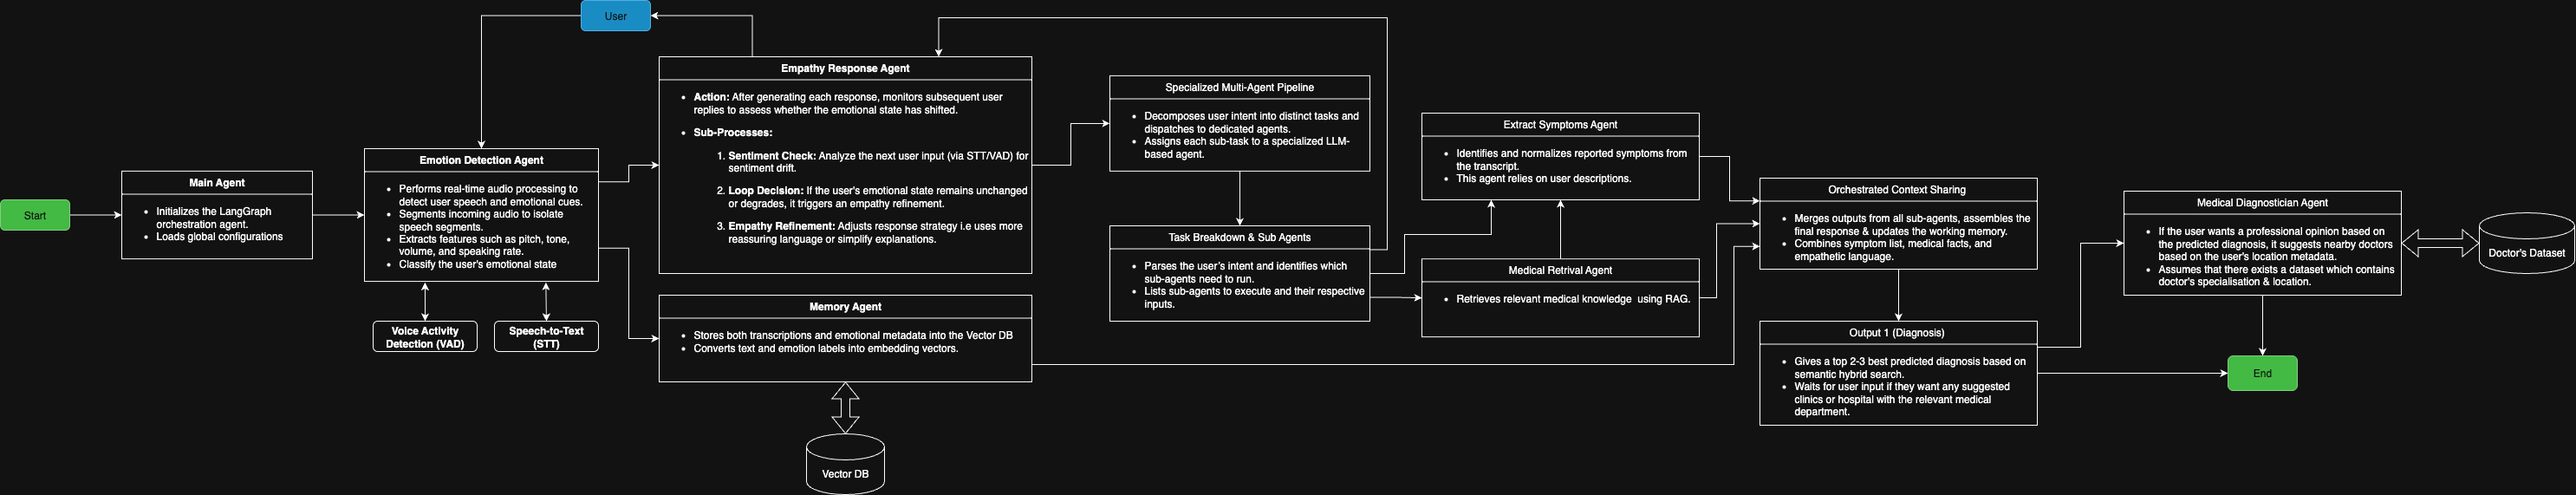
\includegraphics[height=0.31\textheight]{ChatBot_Healthcare_flow.png}
  \caption{Agentic Chatbot System Architecture (Rotated)}
  \label{fig:architecture}
\end{figure}
\end{landscape}

\subsection{High‐Level Flow}
\begin{enumerate}[left=0pt]
  \item User speaks or types input.
  \item Emotion Detection Agent: VAD $\to$ STT $\to$ paralinguistic analysis.
  \item Memory Agent: Ingests transcript + emotion tags into vector DB.
  \item LangGraph Orchestration: Decomposes request, dispatches sub‐agents in parallel.
  \item Symptoms Extraction $\to$ Medical Retrieval (RAG lookup).
  \item Empathy Response Generation with iterative sentiment loop.
  \item Diagnosis presentation + doctor recommendation + booking.
  \item Feedback loop: Next user utterance rescored for sentiment drift.
\end{enumerate}

\subsection{Key Modules}
\begin{longtable}{@{}p{0.25\textwidth}p{0.70\textwidth}@{}}
\toprule
\textbf{Module} & \textbf{Responsibility} \\
\midrule
STT \& VAD & Convert speech to text; detect voice activity, pitch, tone, and pauses. \\
Emotion Detection Agent & Classify valence/arousal; trigger empathy refinement if distress persists. \\
Memory Agent & Store multimodal embeddings in vector DB; support retrieval‐augmented prompts. \\
LangGraph Orchestrator & Define agent graph; handle task decomposition, parallelism, context sharing, and fallbacks. \\
Symptoms Extraction Agent & Normalize free‐form input into structured symptom lists. \\
Medical Retrieval Agent & Query curated clinical guidelines and disease ontologies via RAG. \\
Empathy Response Agent & Generate responses modulated by real‐time emotion checks. \\
Appointment Booking & Suggest specialists (geolocation + doctor dataset); integrate scheduling APIs. \\
\bottomrule
\end{longtable}

\section{Core Features \& User Experience}
\begin{itemize}[left=0pt]
  \item \textbf{Emotion‐Adaptive UX:} On‐screen emotion meter, seamless shifting between technical and empathetic modes.
  \item \textbf{Persistent Medical History \& Emotions:} Recall past diagnoses, medications, and emotional context for tailored follow‐ups.
  \item \textbf{Symptom‐to‐Diagnosis Pipeline:} NL symptom extraction $\to$ RAG lookup $\to$ top‐N differential diagnoses with confidence scores.
  \item \textbf{Doctor Recommendation \& Booking:} From symptom report to scheduled appointment in three conversational turns.
\end{itemize}

\section{Technology Stack}
\begin{tabular}{@{}ll@{}}
\toprule
\textbf{Layer}              & \textbf{Technology} \\
\midrule
Orchestration              & LangGraph \\
LLM APIs                   & OpenAI GPT‐4, Anthropic Claude \\
Speech Modules             & WebRTC VAD, Whisper STT, Amazon Polly / Azure TTS \\
Vector Memory              & FAISS or Pinecone \\
Backend Framework          & Python, FastAPI, Docker, Kubernetes \\
Databases                  & PostgreSQL, Redis, Vector DB \\
Frontend                   & React (Web), Native Mobile SDKs \\
Monitoring \& Logging       & Prometheus, Grafana, ELK \\
Scheduling API             & Calendly; Hospital Scheduling Services \\
\bottomrule
\end{tabular}

\section{Scalability, Security \& Privacy}
\begin{itemize}[left=0pt]
  \item \textbf{Horizontal Scaling:} Containerized LangGraph workflows, Kubernetes HPA.
  \item \textbf{Failover \& Redundancy:} Multi‐region LLM endpoints; fallback to local models.
  \item \textbf{Data Privacy:} HIPAA/GDPR compliance; end‐to‐end encryption; user controls for memory management.
\end{itemize}

\section{Next Steps \& Prototype Plan}
\begin{enumerate}[left=0pt]
  \item \textbf{MVP (6 weeks):} Core STT $\to$ Emotion tagging $\to$ LangGraph orchestration $\to$ symptom extraction $\to$ RAG $\to$ simple empathy loop; basic UI.
  \item \textbf{Pilot Testing (4 weeks):} 20‐user trial; validate emotion accuracy (target ≥80\% human agreement); appointment flow usability.
  \item \textbf{Iteration (8 weeks):} Add parallel multi‐model generation, advanced empathy refinements, admin memory dashboard, full scheduling integration.
\end{enumerate}

\section{Conclusion}
Our proposed architecture—combining multimodal emotion memory, a LangGraph agent pipeline, and RAG‐powered medical retrieval—yields an empathetic, accurate, and action‐oriented healthcare chatbot. We look forward to prototyping and demonstrating its impact on patient engagement and care efficiency.

\end{document}
